% MSc thesis style for TU Delft Embedded Networked Systems Group.

% MIT License
%
% Copyright (c) 2023 TU Delft Embedded Systems Group and Casper Dennis van Wezel.
%
% Permission is hereby granted, free of charge, to any person obtaining a copy
% of this software and associated documentation files (the "Software"), to deal
% in the Software without restriction, including without limitation the rights
% to use, copy, modify, merge, publish, distribute, sublicense, and/or sell
% copies of the Software, and to permit persons to whom the Software is
% furnished to do so, subject to the following conditions:
%
% The above copyright notice and this permission notice shall be included in all
% copies or substantial portions of the Software.
%
% THE SOFTWARE IS PROVIDED "AS IS", WITHOUT WARRANTY OF ANY KIND, EXPRESS OR
% IMPLIED, INCLUDING BUT NOT LIMITED TO THE WARRANTIES OF MERCHANTABILITY,
% FITNESS FOR A PARTICULAR PURPOSE AND NONINFRINGEMENT. IN NO EVENT SHALL THE
% AUTHORS OR COPYRIGHT HOLDERS BE LIABLE FOR ANY CLAIM, DAMAGES OR OTHER
% LIABILITY, WHETHER IN AN ACTION OF CONTRACT, TORT OR OTHERWISE, ARISING FROM,
% OUT OF OR IN CONNECTION WITH THE SOFTWARE OR THE USE OR OTHER DEALINGS IN THE
% SOFTWARE.

\documentclass[10pt,twoside,a4paper,openright]{report}

% add new packages here


% math packages
\usepackage{amsmath}
\usepackage{amssymb}

% textblocks for title page
\usepackage[absolute]{textpos}

% use babel for proper hyphenation
\usepackage[british]{babel}

% Graphics: different for pdflatex or dvi output, choose one
%%\usepackage[dvips]{graphicx}
%%\usepackage[pdftex]{graphicx}
\usepackage{graphicx}

\usepackage{epstopdf}
\usepackage{rotating}
% \usepackage{subfigure} old package, subcaption is better

% Make captions distinguishable
\usepackage[textfont=bf]{caption}

% Chose font style
\usepackage[scaled=.92]{helvet}
\usepackage[T1]{fontenc} % to allow symbols like < and >

% for url's use "\url{http://www.google.com/}"
\usepackage{url}
\usepackage[plainpages=false]{hyperref} 

% [[ BRENDAN PACKAGE ]]
\usepackage{wrapfig} % Allows for figures inside of text
\usepackage{subcaption} % Subfigures and such
\usepackage[export]{adjustbox}

% [[ natbib with `plain` looks]]
% The paper wants me to use the "plain" bibliography style, but I'd really like the features form 
% the `natbib` package, this setup should do exactly that
\usepackage[numbers,sort&compress]{natbib} % Load natbib in numeric mode (same as plain)
\setcitestyle{square,comma,numbers,sort&compress} % enforce exact same bracket/comma style as plain.bst

\usepackage{textcomp, gensymb} % Mathematical symbols, such as the degree ( ° ) symbol

\usepackage{cleveref} % Automatically references well.
% Define a new command for appendix chapters



% Information that will be filled in at various points in the report
\newcommand{\reportTitle}{WRITE YOUR THESIS TITLE HERE}
\newcommand{\reportAuthor}{Brendan Rudolf Mesters} % Please put your full and official name here: no abbreviations (and to Dutch students: geen roepnamen)
\newcommand{\studentNumber}{4876016}
\newcommand{\reportEmailTUD}{b.r.mesters@student.tudelft.nl}
\newcommand{\reportEmailNonTUD}{brendanmesters@gmail.com}
\newcommand{\reportUrlEmailTUD}{\href{mailto:\reportEmailTUD}{\reportEmailTUD}}
\newcommand{\reportUrlEmailNonTUD}{\href{mailto:\reportEmailNonTUD}{\reportEmailNonTUD}}
\newcommand{\reportMSC}{Computer and Embedded Systems Engineering} % Examples are {Embedded Systems} {Computer Engineering} {Computer Science} or {Electrical Engineering}
\newcommand{\reportDate}{PUT DATE OF PROVIDING THESIS TO GRADUATION COMMITTEE HERE}
\newcommand{\presentationDate}{PUT DATE OF YOUR PRESENTATION HERE}
\newcommand{\graduationCommittee}{
PUT THE NAME AND SURNAME OF GRADUATION COMMITTEE MEMBER 1 HERE & Delft University of Technology \\
PUT THE NAME AND SURNAME OF GRADUATION COMMITTEE MEMBER 2 HERE & Delft University of Technology \\
% ...
PUT THE NAME AND SURNAME OF GRADUATION COMMITTEE MEMBER X HERE & Delft University of Technology \\
}

% Provide full name and surname (no abbreviations), so "Koen Langendoen" not "K. Langendoen"

% The order of listing above: 

% title + Graduation committee chairman name and surname (chairman)
% title + Supervisor 1 name and surname (direct supervisor)
% title + Supervisor 2 name and surname (direct supervisor)
% ...
% title + Supervisor X name and surname (direct supervisor) 
% ...
% Others (ordered by title and alphabetical)

% Example: 
% prof.\,dr.\,Koen Langendoen (chairman) & Delft University of Technology \\ 
% dr.\,Przemys{\l}aw Pawe{\l}czak & Delft University of Technology \\ 

\newcommand{\reportAbstract}{WRITE YOUR ABSTRACT HERE}

\newcommand{\reportKeywords}{LIST YOUR KEYWORDS HERE}

% Did the thesis lead to a paper? 
% e.g. The work presented in this thesis has lead to a paper which has been submitted to a conference for publication, pending peer-review
%\newcommand{\reportPaper}{LINE ABOUT YOUR PUBLICATION GOES HERE}
\newcommand{\reportPaper}{}


% Information for pdflatex
\pdfinfo{
/Author (\reportAuthor)
/Title (\reportTitle)
/Keywords (\reportKeywords)
}

\begin{document}


\pagenumbering{alph}
\pagestyle{empty}

% Make frontcover
% MSc thesis style for TU Delft Embedded Networked Systems Group.

% MIT License
%
% Copyright (c) 2019 TU Delft Embedded and Networked Systems Group and Casper Dennis van Wezel.
%
% Permission is hereby granted, free of charge, to any person obtaining a copy
% of this software and associated documentation files (the "Software"), to deal
% in the Software without restriction, including without limitation the rights
% to use, copy, modify, merge, publish, distribute, sublicense, and/or sell
% copies of the Software, and to permit persons to whom the Software is
% furnished to do so, subject to the following conditions:
%
% The above copyright notice and this permission notice shall be included in all
% copies or substantial portions of the Software.
%
% THE SOFTWARE IS PROVIDED "AS IS", WITHOUT WARRANTY OF ANY KIND, EXPRESS OR
% IMPLIED, INCLUDING BUT NOT LIMITED TO THE WARRANTIES OF MERCHANTABILITY,
% FITNESS FOR A PARTICULAR PURPOSE AND NONINFRINGEMENT. IN NO EVENT SHALL THE
% AUTHORS OR COPYRIGHT HOLDERS BE LIABLE FOR ANY CLAIM, DAMAGES OR OTHER
% LIABILITY, WHETHER IN AN ACTION OF CONTRACT, TORT OR OTHERWISE, ARISING FROM,
% OUT OF OR IN CONNECTION WITH THE SOFTWARE OR THE USE OR OTHER DEALINGS IN THE
% SOFTWARE.

\begin{textblock*}{210mm}(0mm,0mm)
\noindent
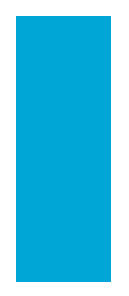
\includegraphics[height=3.2cm]{template-pics/block} % Blue rectangle on top, left side, of front page
\sffamily
\vspace{.8cm}

\begin{center}

\Large
Delft University of Technology\\
Master of Science Thesis in \reportMSC\\
\vspace{2cm}
\parbox{170mm}{\bfseries\centering\Huge\reportTitle}\\
\vspace{1cm}
\parbox{170mm}{\bfseries\centering\reportAuthor}

\end{center}
\end{textblock*}

\begin {textblock*}{210mm}[0.0,1.0](0mm,297mm)
\noindent
\hspace{1.89cm}

\hfill\parbox{5cm}{
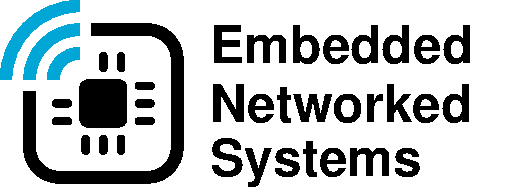
\includegraphics[width=5cm]{template-pics/tud-ens-logo-tikz/tud-ens-logo}} % TU Delft ENS Logo inTikZ format: please compile tud-ens-logo.tex first if tud-ens-logo.pdf does not exist
\hspace*{2cm}\\

\vspace*{1.5cm}
\noindent

\includegraphics[width=\textwidth]{template-pics/TU_border_A4_L_front} % Footer with logo
\end{textblock*}

\null\newpage

% Set marginns
\hoffset=1.63cm
\oddsidemargin=0in
\evensidemargin=0in
\textwidth=5in

%
\parindent=1em

% Empty page
\cleardoublepage

\pagestyle{plain}
\pagenumbering{roman}
\setcounter{page}{1}


% Create title page: page i (hidden)
% MSc thesis style for TU Delft Embedded Networked Systems Group.

% MIT License
%
% Copyright (c) 2019 TU Delft Embedded and Networked Systems Group and Casper Dennis van Wezel.
%
% Permission is hereby granted, free of charge, to any person obtaining a copy
% of this software and associated documentation files (the "Software"), to deal
% in the Software without restriction, including without limitation the rights
% to use, copy, modify, merge, publish, distribute, sublicense, and/or sell
% copies of the Software, and to permit persons to whom the Software is
% furnished to do so, subject to the following conditions:
%
% The above copyright notice and this permission notice shall be included in all
% copies or substantial portions of the Software.
%
% THE SOFTWARE IS PROVIDED "AS IS", WITHOUT WARRANTY OF ANY KIND, EXPRESS OR
% IMPLIED, INCLUDING BUT NOT LIMITED TO THE WARRANTIES OF MERCHANTABILITY,
% FITNESS FOR A PARTICULAR PURPOSE AND NONINFRINGEMENT. IN NO EVENT SHALL THE
% AUTHORS OR COPYRIGHT HOLDERS BE LIABLE FOR ANY CLAIM, DAMAGES OR OTHER
% LIABILITY, WHETHER IN AN ACTION OF CONTRACT, TORT OR OTHERWISE, ARISING FROM,
% OUT OF OR IN CONNECTION WITH THE SOFTWARE OR THE USE OR OTHER DEALINGS IN THE
% SOFTWARE.

\begin{titlepage}

\begin{center}
\null\vfill
\begin{center}
\LARGE{\reportTitle}
\end{center}

\vspace{3cm}

\begin{large}
Master of Science Thesis in \reportMSC
\end{large}

\vspace{1.5cm}

\begin{normalsize}
Embedded and Networked Systems Group\\
Faculty of Electrical Engineering, Mathematics and Computer Science\\
Delft University of Technology\\
Mekelweg 4, 2628\,CD Delft, The Netherlands
\end{normalsize}

\vspace{2.0cm}

\begin{normalsize}
\reportAuthor \\
\reportUrlEmailTUD \\
\reportUrlEmailNonTUD\\
\textbf{TU Delft Student Number:} \studentNumber
\end{normalsize}

\vspace{1.0cm}

\reportDate

\vfill
\end{center}

\end{titlepage}

% Create Graduation Data and Abstract: pages ii and iii (hidden)
% MSc thesis style for TU Delft Embedded Networked Systems Group.

% MIT License
%
% Copyright (c) 2019 TU Delft Embedded and Networked Systems Group.
%
% Permission is hereby granted, free of charge, to any person obtaining a copy
% of this software and associated documentation files (the "Software"), to deal
% in the Software without restriction, including without limitation the rights
% to use, copy, modify, merge, publish, distribute, sublicense, and/or sell
% copies of the Software, and to permit persons to whom the Software is
% furnished to do so, subject to the following conditions:
%
% The above copyright notice and this permission notice shall be included in all
% copies or substantial portions of the Software.
%
% THE SOFTWARE IS PROVIDED "AS IS", WITHOUT WARRANTY OF ANY KIND, EXPRESS OR
% IMPLIED, INCLUDING BUT NOT LIMITED TO THE WARRANTIES OF MERCHANTABILITY,
% FITNESS FOR A PARTICULAR PURPOSE AND NONINFRINGEMENT. IN NO EVENT SHALL THE
% AUTHORS OR COPYRIGHT HOLDERS BE LIABLE FOR ANY CLAIM, DAMAGES OR OTHER
% LIABILITY, WHETHER IN AN ACTION OF CONTRACT, TORT OR OTHERWISE, ARISING FROM,
% OUT OF OR IN CONNECTION WITH THE SOFTWARE OR THE USE OR OTHER DEALINGS IN THE
% SOFTWARE.

\thispagestyle{empty}

\noindent \textbf{Author}\\
\begin{tabular}{l}
\reportAuthor{} (\reportUrlEmailTUD)\\ (\reportUrlEmailNonTUD)\\ (\textbf{TU Delft Student Number:} \studentNumber)
\end{tabular}\\
\noindent \textbf{Title}\\
\begin{tabular}{l}
\reportTitle\\
\end{tabular}\\
\noindent \textbf{MSc Presentation Date}\\
\begin{tabular}{l}
\presentationDate\\
\end{tabular}

\vspace{1.1cm}

\noindent \textbf{Graduation Committee}\\
\begin{tabular}{ll}
\graduationCommittee
\end{tabular}

\begin{abstract} 
\setcounter{page}{3}
\reportAbstract{}
\end{abstract}

\clearpage

% Empty page: page iv
\cleardoublepage

% (Optional) Include quotation: page v (uncomment if needed)
\pagestyle{empty}

\null\vfill

\begin{center}
\emph{``WRITE YOUR QUOTE HERE''} -- WRITE THE NAME OF THE AUTHOR OF THE QUOTE HERE
\end{center}

\vspace{10cm}

\clearpage

% Empty page: page vi
\cleardoublepage

% Create preface: page v
\chapter*{Preface}
\addcontentsline{toc}{chapter}{Preface}

Put a motivation for a research topic here.

\vspace{1\baselineskip}

Put acknowledgments here.

\vspace{1\baselineskip}

\reportAuthor

\vspace{1\baselineskip}

\noindent
Delft, The Netherlands

\noindent
\today

% Empty page: page vi
\cleardoublepage

% Create tabe of contents: page vii
\tableofcontents

\cleardoublepage

\pagenumbering{arabic}
\setcounter{page}{1}

% Create Introduction: page 1
% \chapter{Introduction}
\label{chp:introduction}

Introduction goes here.
\chapter{Introduction}
\label{chapter: introduction}


This century, we have seen computers become more and more integrated into our everyday environment, and as such, the user interfaces of the past might not be suitable for all these systems anymore.
Many systems are not a "dedicated tool" anymore, such as the home computer, but rather an integrated part of your environment, think smart lamps, or voice assistants.
It is not always practical to control these systems with dedicated and noticeable input devices, such as a keyboard, mouse, or tablet.
Many such systems use someone's smartphone as an interface, or use voice commands to control these devices, however, those are not the only options available.
This thesis provides an example interface to a musical application, which senses the user's body and reacts to its movement in a privacy-preserving manner.
Similar systems have been built before, using the same sensor technology, but these previous systems relied on deep learning models, which are prone to overfitting, may need extensive retraining in new environments, and require an impractical amount of training data to produce good results.
This thesis sets out to design a Human Pose Estimation (HPE) system, using a Millimeter Wave (MMWave) sensor, which relies solely on explainable, debuggable, and tunable algorithms.

\section{Motivation}
\label{section: introduction - motivation}

Computers are getting more and more integrated into our everyday lives, from smart watches to voice-controlled house assistants, from electric cars to IOT houses.
Therefore, it's important to explore robust, intuitive, and power-efficient interfaces to these systems.

\section{Research Challenge}
\label{section: introduction - research challenge}

In this thesis, we will explore the possibility of algorithmic interpretation methods of mmWave point clouds.
We will design a system which can predict the general position of a users arms, into one of three distinct regions, "low", meaning angled at ...., "middle", which is the region of angles ...., and high, given the region of angles ....



\section{Scientific Gap}
\label{section: introduction - scientific gap}

% All of the current research into HPE with MMWave radars has used Deep Learning (DL) algorithms for data interpretation, and research into algorithmic interpretation is very lacking.
% Deep learning has many strengths, but also many weaknesses, as such, I believe it 

I will talk about the current focus which MMWave HPE research has on Deep Learning, and the scientific gap which exists in non-DL methods.
I'll want to discuss the problems and shortcommings of DL methods.
I also want to talk about the potential benefits which stochastic methods would have: 
% reason 1
Lower power consumption, lower computer resource consumption; 
% reason 2
More room for manual tuning to new environments, as opposed to training on new data (which takes a lot more work); 
% reason 3
The potential for "reasoning" about the good and the bad results, and improving based on that

Due to the aforementioned I think its very useful to explore algoritmic data interpretation systems, since these would be more stable, less resource hungry, and could offer a better basis for any HPE applications.
% Here I'll also lay out my envisoined system, which uses stochastic methods to find the angle of someones arms, while \textbf{briefly} mentioning the example musical application.


% \section{Background}
\label{section: introduction - background}

\textbf{¿¿¿ Should this be a section or a chapter ???}

This thesis works with a specific sensor, the Millimeter Wave Radar (MMWave Radar), and tries to solve a specific problem, Human Pose Estimation (HPE). 
This section aims to give readers the necessary knowledge on these subjects to be able to read and understand this thesis.
Furthermore, we will discuss some of the current state-of-the-art systems for HPE using an MMWave radar.

% I'll give background on MMWave, HPE, and the current SOA HPE methods used with MMWave.
% I will also discuss some of the properties of MMWave which makes it difficult to handle

\subsection{Millimeter Wave Radar}
\label{sub-section: introduction - background - millimeter wave radar}
Give an explanation of what MMWave radars are, to what extent we can configure them, and what we get out of them (3d pointclouds, at ~10Hz, with between 30-100 points per frame).
Mention the inherent privacy-preserving nature of MMWave due to its not capturing images, and how it fares better in varied light conditions (overexposure/underexposure).
Also, briefly explain how they work internally, using \textit{beam forming antennas} on the receiving and, as well as the large amount of FFT's over the raw signal, to get to pointclouds.

I should mention that the data from MMWave radars is not always temporally stable.
Aka, one frame I might see my left arm, but the next I might see my right.
This is important for section \cref{sub-section: methodology - data filtering - temporal filtering}.

\subsection{Human Pose Estimation}
\label{sub-section: introduction - background - human pose estimation}
Explain what exactly human pose estimation is, and reference some papers discussing it. 
Present the kinect and skeletal estimation, and \textbf{clearly specify} the \textbf{differences} between my \textit{arm location} estimation, and a \textit{full skeletal estimation}.

\subsection{Current State of the Art}
\label{sub-section: introduction - background - current soa}
Briefly mention some \textit{non-mmwave} HPE solutions, those using cameras and those using sensors, as well as their shortcomings (privacy/light situation and clunkiness of wearables, respectively).
Discuss the various SOA MMWave HPE sollutions, their strengths, weaknesses and shortcommings.
Also specify the strengths of Stochastic explainable systems over DL systems (tunable, testable, explainable, significantly lower need for training data), and setup a bridge to the scientific gap.



% \input{sections/1. introduction/1.2. scientific gap}

% \input{sections/1. introduction/1.3. objective}

% \input{sections/1. introduction/1.4. significance of the research}

% \input{sections/1. introduction/1.5. upcomming chapters}


% Create a chapter for backgorund and related work
\chapter{Background}
\label{chapter: background}

This thesis aims to create an algorithmic interpretation method for the point clouds generated by \textit{millimeter wave radars} (\textbf{mmWave Radars}), which is both \textit{explainable} and \textit{tunable}.
This method will interpret data for the purpose of \textit{human pose estimation} (\textbf{hpe}), a task which has thus far only been explored with the use of \textit{deep learning} (\textbf{dl}) systems.
This chapter should provide sufficient background knowledge to understand this thesis and will provide a clear view of existing research which is related to the research question of this thesis.

% This thesis works with a specific sensor, the Millimeter Wave Radar (mmWave Radar), and tries to solve a specific problem, Human Pose Estimation (HPE). 
% This section aims to give readers the necessary knowledge on these subjects to be able to read and understand this thesis.
% Furthermore, we will discuss some of the current state-of-the-art systems for HPE using an MMWave radar.


\section{Millimeter Wave Radar}
\label{section: background - millimeter wave radar}
Give an explanation of what MMWave radars are, to what extent we can configure them, and what we get out of them (3d pointclouds, at ~10Hz, with between 30-100 points per frame).
Mention the inherent privacy-preserving nature of MMWave due to its not capturing images, and how it fares better in varied light conditions (overexposure/underexposure).
Also, briefly explain how they work internally, using \textit{beam forming antennas} on the receiving and, as well as the large amount of FFT's over the raw signal, to get to pointclouds.

I should mention that the data from MMWave radars is not always temporally stable.
Aka, one frame I might see my left arm, but the next I might see my right.
This is important for section \cref{sub-section: methodology - data filtering - temporal filtering}.



\section{Human Pose Estimation}
\label{section: background - human pose estimation}
Explain what exactly human pose estimation is, and reference some papers discussing it. 
Present the kinect and skeletal estimation, and \textbf{clearly specify} the \textbf{differences} between my \textit{arm location} estimation, and a \textit{full skeletal estimation}.



\section{algorithmic pointcloud methods?}
\label{section: background - algorithmic pointcloud methods}

This thesis is, for a large part, based on a comparison between deep learning methods and algorithmic methods, both of which have advantages and disadvantages.
A large advantage of algorithmic systems is that they can be reasoned about and can be configured in a clear manner with the use of input parameters.
For pointcloud analysis, some great and concise clustering algorithms have been created, such as DBSCAN \cite{ester1996dbscan}, and some problems are being successfully tackled by both DL systems, as well as algorithmic systems, such as geometric labeling of pointcloud data \cite{poux2019voxel}, or audio reconstruction using mmWave radars \cite{li2025acoustic}.



% A part of the different algorithmic methods to handle large swaths of high-dimensional data, specifically for clustering.
% This has gotten a lot of recent attention due to Machine Learning implementations often transforming data into a high-dimensional space.

% \textbf{DBSCAN signal processing algorithm} \cite{ester1996dbscan}\\
% \textbf{SOA acoustic reconstruction system} \cite{li2025acoustic}

\section{Related Work}
\label{section: background - related work}

% [[ Broad background ]]
% - Deep Learning
% - HPE
% - Pointclouds


% [[ Narrowing ]]
% - mmWave
% - pointcloud DL systems
% - algorithmic pointcloud processing (DBSCAN, tracking, etc)

% [[ Specific ]]
% - mmWave HPE SOA
% - simpler models (MARS) and more complex models (???)
% - no existing algorithmic mmwave hpe methods.

Generic point cloud algorithms

Early and more recent HPE methods (camera, wearable, wifi, mmwave)

DL vs algorithmic solutions

algorithmic mmWave/pointcloud solutions: DBSCAN, etc

HPE with mmwave (the DL systems, including mars)

Algorithmic HPE for mmWave pointclouds \textbf{does not yet exist}

\subsection{Current State of the Art}
\label{sub-section: background - related work - current soa}
Briefly mention some \textit{non-mmwave} HPE solutions, those using cameras and those using sensors, as well as their shortcomings (privacy/light situation and clunkiness of wearables, respectively).
Discuss the various SOA MMWave HPE sollutions, their strengths, weaknesses and shortcommings.
Also specify the strengths of Stochastic explainable systems over DL systems (tunable, testable, explainable, significantly lower need for training data), and setup a bridge to the scientific gap.


% Create a set discussing the tracking methods
\chapter{Tracking Method}
\label{chapter: tracking method}

The main goal of the thesis is to find a method for predicting \textit{where} a user's arms are located, from a pointcloud generated by a millimeter wave radar.
More specifically, it should tell us in what general \textbf{zone} the arm is currently present, this can be either: 
"low", where the user's arm points at the ground;
"middle", where the user's arm points out to the side;
or "high", where the user's arm points up to the sky.
These regions exist both for the left and for the right arm, and thus there are 6 different \textit{zones} which the system tries to predict.
There are, of course, some physical bounds on this model. 
A person can, for example, only have their arm in \textit{one zone}, that means the system will always output \textbf{one} \textit{left zone} (left low; left middle; left high) and \textbf{one} \textit{right zone}.

To facilitate this "zone detection", a standalone pipeline was built to handle the whole process from communication with the FMCW and package decoding, through to the filtering, labeling, and interpretation of the data. 
In this report, we will focus on the latter part of this pipeline, which implements this paper's interpretation algorithm.
The final system used by IAmMuse will be discussed in \cref{section: tracking method - data enhancement}
 and \cref{section: tracking method - data interpretation}.
The final pipeline for IAmMuse only arrived after a lot of different approaches had been explored and proved unfruitful.
These approaches are briefly discussed in \cref{app: failed methods}.

% After that, \cref{section: tracking method - different approaches} will discuss some of the earlier attempts, as well as reasoning why those might have failed.

The IAmMuse system, as well as most later approaches, uses a workflow where the final \textit{interpretation} system relies on an \textit{initialization} performed by the user.
During the creation of IAmMuse, it was found that it was not feasible to interpret the MMWave data without any sort of context.
Such an \textit{initialization} step may not be needed in the future, as the understanding of effective interpretation methods improves, these steps could feasibly be done in real time, during usage.
However, creating such an understanding of effective methods of generating context of a pointcloud does benefit greatly from a well-defined initialization step, for that reason, IAmMuse chose to use such an initialization step.

\section{Data filtering}
\label{section: tracking method - data filtering}

One issue present with the MMWave Sensors (in our experience) is the fact that they are susceptible to both environmental noise as well as seemingly random noise. 
This noise often occurred in "streaks", lines of points through your 3d space. 
These "streaks" were not very dense spatially and usually only existed for a single frame.
Due to these attributes, a combination of a temporal as well as a spatial filter was used to filter out the noise points.

For this section, it's useful to know that the MMWave produces roughly 10 frames per second, thus each frame is roughly 100 ms.

\subsection{Spatial Filtering}
\label{sub-section: tracking method - data filtering - density filtering}

A very common strategy for filtering spatial data is to look at the density and internal cohesion between points.
The main idea on which this is based is the assumption that points with \textit{many close neighbors} are likely to \textit{represent reality well}, a "strength in numbers" kind of philosophy.
In our system, the \textit{spatial filter} looks on a \textit{frame by frame basis} at the clustering of the points.
Each point then gets assigned a value based on the cumulative weight of its neighbors (distance < 25 cm). 
Based on this value, points can be labelled as "noise" or "signal".

The main function of spatial filtering is to remove outliers, to always let large clusters pass, and to give an indication of how important any sparse clusters are.
By using the cumulative weight of the neighbours of a point, we also ensure that points which have already been shown to be more likely to be of use will be disproportionately selected.
One type of noise that the spatial filtering does not handle well, however, is dense but brief noise spikes, since our spatial filtering method only takes into account a single frame.
That is why the system also uses \textit{temporal filtering}.

% We also filter on the density in a single frame, since high in-frame consistency also often shows high quality of the data.
% However, sometimes noise streaks are dense enough to falsely trigger this system.


\subsection{Temporal Filtering}
\label{sub-section: tracking method - data filtering - temporal filtering}
The main function of the \textit{temporal filter} in this system is to provide stability across frames and to detect and remove noise spikes.
The temporal filter achieves this in a very similar way to the spatial filter, but instead of considering other points in the same frame, it only considers points in previous frames.
More specifically, the temporal filter takes into consideration the three frames (0.3-0.4 seconds) which came before, it then gives each point a score equal to the cumulative weight of spatially nearby points (within 20 cm) within these prior frames.
This means that points in a dense cloud may all get a very low score if little or no data has been found in that area recently.
In this way, the \textit{temporal filter} can 'punish' any inconsistent data, such as sudden but dense noise spikes.

Removing inconsistent data is not the only thing which the temporal filter does.
The temporal filter also 'rewards' points in a very stable area more than the density filter would, because the temporal filter takes into account points of three different frames.
This means that any data which is consistently present in an area across frames will be highly rated by the temporal filter, even though it takes into account a slightly smaller neighbourhood (20 cm as opposed to the 25 cm of spatial filters).
That being said, on their own, temporal filters can often miss large amounts of data, since the MMWave sensor does not always produce temporally consistent data, as discussed in \cref{sub-section: introduction - background - millimeter wave radar}.
That is why the actual system uses a combination of both a \textit{spatial} and a \textit{temporal} filter.


% Temporal data filtering was chosen, as the noise most often encountered was only present in a single frame. 
% By comparing the points in subsequent frames, these noise points can be filtered out by looking at the stability across frames.
% This was implemented by checking the number of neighbours on different frames that any point had within a specified distance (e.g., 10 cm). 
% In this case, even dense clusters on a single frame will be filtered out if this cluster is not present on other frames.
% 
% A danger of this approach is that you might lose correct points, this problem becomes more prevalent if the data is not always consistent over time.
% If the FMCW measures an arm (so not noise) in frames 1, 3, and 5, all that data will be discarded if we only consider a window of 3 frames (centred on the frame to be looked at, so on frame 3, we consider frame 2, 3, 4).
% Due to this side effect, it's important to choose the \textit{window of frames} you consider, as well as the \textit{minimum number of neighbours} and the \textit{distance within which you count as a neighbour}.


\subsection{Combined Filtering and Tuning}
\label{sub-section: tracking method - data filtering - combined filtering and tuning}

The system uses a combination of the \textit{spatial} and the \textit{temporal} filters, where it combines their respective scores, to make use of the strengths of both, while mitigating the weaknesses of both.
The combined filter has six variables which it can tune: the number of frames considered in the temporal system; for both the \textit{spatial} \textbf{and} the \textit{temporal}, the neighbourhood size considered, and the threshold cumulative weight to distinguish between noise an signal; and lastly the amount we take into account the spatial result or the temporal result.
Combining these two systems, however, does make it more difficult to tune, as there are more moving parts.
Therefore, a specific tuning strategy was thought up beforehand to get the system to a reasonable state. Afterwards, small tweaks were still made, based on what looked good to the visual inspection of the researcher.
% This is the main reason why we made a specific tuning strategy for this system before we started actually tuning it, though some manual tuning was still required in the end.

The tuning strategy which was used for this system was based on two principal ideas, namely, that the spatial filtering would be best at getting our positive values, while still avoiding some outliers and that the temporal filter would be able to provide enough of a counterbalance to mark inconsistent points as noise, while keeping the consistent points to be signal.
Our tuning strategy is thus to start by tuning the \textit{spatial filter} on its own in such a way that it captures all points we deem to be part of the signal, this means that it will also capture some points which are deemed to be noise (by the researcher).
Then the \textit{temporal filter} should be tuned, once again on its own, in such a way that it must not capture any noise, even if this means missing some points which are part of the signal.
These two filters are then combined (starting with a 50-50 split of effectiveness), and fine-tuning will happen. 
Here, the various variables will be modified slowly to resolve problems which are encountered.
In general, if signal points are missed, we should want either to increase the neighbourhood size of the spatial filter, lower its threshold, or make it more prevalent in the filter split.
In a similar vein, if noise points are not identified as such, we will want to increase the prevalence of the temporal filter in the filter split, lower the temporal threshold, or decrease its neighbourhood size.

A big advantage of this system is that it can be quickly tuned to the specific scenario, since the output of MMWave sensors can differ quite drastically based on the physical setup of the sensor and its environment.
This means that a system can be moved around with relatively little effort when you compare it to systems based on deep learning.
If you have a good quality metric for a point cloud recording, e.g. you want a lot of points and the points should be stable, you might even be able to automate it due to the low number of input parameters.

% Combined filters aim to make use of the best of both filters while mitigating the weaknesses of both filters.
% Tuning such a system is always an important part, the way this system was tuned was by first loosely tuning both systems, keeping in mind what we want from them.

% The density filter was tuned in such a way that it would recognise most actual hand recordings (with any significant number of points, e.g. 5-7 min) while letting through as few noise streaks as we can.

% The temporal filter was filtered in such a way that it notices a decent number of hand positions, while prioritising filtering out noise streaks.

% So density should catch almost all hands, while temporal should ignore almost all noise.

% During the combination of both filters, we want to give enough weight to temporal filter, to remove most noise streaks, but we want to not make it to great, so that we still recognize hand clusters which are only "good visible" in one frame.

% We tune the individual filters with Distance (for neighber search) and threshold neighber value. And for temporal, we also use the number of frames considered (values between 3-7 where considered, though any number > 5 (~half a second) already risks being more noise then data).
% Lastly we ofcourse have to decide in what manner we want to combine both.

% The advantage of doing it this way is that you can "retune" if you're tackeling a different scenario. e.g. a scenario with slow moving hands will probably want to consider a higher number of frames, while one with fast moving hands wants to consider less frames. So too you can make density filters more prevalent in your final filter if you don't encounter a lot of random noise, while you can lean more on temporal filters if you are.


\section{Data Enhancement}
\label{section: tracking method - data enhancement}


The data that comes from the mmWave sensor is quite sparse, thus, it's important to get as much information out of this data as we can, this process is called \textit{data enhancement}.
Data enhancement broadly covers any method that increases the "\textit{quality}" of the data that is being sent to the recognition systems.
This can be done in two major ways: firstly, the physical setup can be changed to increase the quality of the data, secondly, software systems can be put in place to add extra context to the raw data.
The first option, a change to the physical setup, can be quite effective, however, this should be avoided for the final product as it limits the flexibility of the system.
However, physical setup changes can help greatly during the design of a system, as you need good data to design a good interpretation system, and you need a good interpretation system to verify your data enhancement methods.
% One way in which this can be done is by changing the physical setup for the point gathering, though we would like to avoid this for the final product, as this could greatly limit the flexibility of the system.
Software-based data enhancement is more difficult to create, but also more flexible, which makes it a preferable option for the final system.
These systems work by adding additional information to the data already present, this is also where the difference between filtering and data enhancement exists.
Section \ref{section: tracking method - data filtering}, \textit{Data filtering}, also adds information, the label of "noise" vs "signal", but this is a subtractive (removing faulty data) process, as opposed to an additive (adding additional useful data) process, therefore, a distinction between filtering and enhancement is made.

\textbf{add a part about why we want to look at hands?}

\subsection{Physical Enhancement}
\label{sub-section: tracking method - data enhancement - physical enhancement}


Many similar HPE systems rely solely on physical wearables \cite{filippeshi2017survey, antonio2010the}. 
This is a logical choice, as it enables the direct tracking of specific parts of the user's body, at the cost of being more invasive and not easily deployable in non-private spaces.
In IAmMuse, a wearable was chosen that increases the reflectivity of a specific part of the user's body, namely their hands. Increasing the reflectivity
\begin{wrapfigure}{r}{0.32\textwidth}
    \caption{A reflective wearable}
    \centering
    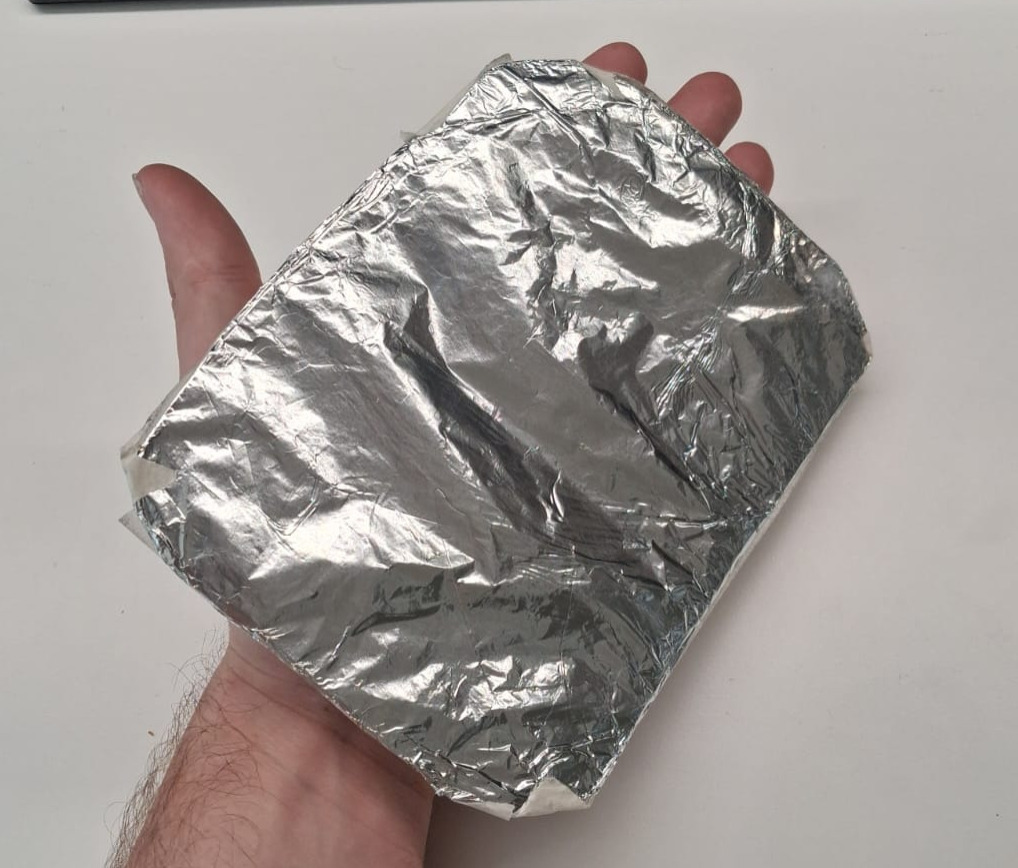
\includegraphics[width=0.32\textwidth]{figures/experimental setup/reflective wearable.png}
    \label{fig: reflective glove wearable}
\end{wrapfigure}
 at a certain location will make the mmWave radar generate more and denser point clusters at that location.
The reason IAmMuse wants a higher point density at the user's hands is due to the fact that the position of the hands is most indicative of the angle of a user's arm.
This is true because, for every angle change at the user's arm, the user's hand will move the largest distance, simply by being the part of the arm furthest removed from the shoulder.
For this reason, the hand is the most effective location to increase the reflectivity and thus point generation.
The software data enhancement method used by IAmMuse will, for the same reason, also increase the prevalence of the points belonging to the user's hands.




% One issue with data enhancement methods is that it's difficult to test enhancement methods if the system using the data does not work well yet, and it's difficult to test that a system is working well without good data enhancement methods.
% For this reason, it was decided that we would use a known \textit{physical} data enhancement method, in the form of a wearable (\cref{fig: reflective glove wearable}).
% This wearable could be worn on the hand and was covered in aluminum foil to increase the reflectivity of the hand.
% This caused the hands to produce more dense pointclouds, since the mmWave radar produces more points for more reflective surfaces.
% This, in turn, is useful since the hands are most indicative of the angle of someone's arm (assuming outstretched arms) as they are furthest away from the shoulder, and thus move the most when someone moves their arm.
% These reflective gloves ensured that the data used to create the later systems was of good quality while they were being designed.

% With the later parts of the pipeline in a decent state, it was possible to create software-based data enhancement methods and to "take off the gloves", so to speak.
% A significant part of this thesis was spent on creating and testing various systems of data enhancement, most of which did not produce adequate results, but which are still discussed in \cref{section: tracking method - different approaches}. 
% Furthermore, many of these systems rely, one way or another, on a "\textit{pre-configuration step}", where the user is asked to perform certain actions at startup for the system to initialize, which is discussed in \cref{section: tracking method - pre configuration}.
% Most of these data enhancement systems tried to "find" which points belonged to the hands, arms, and torso.
% This labeling would allow for weighing points of the hands more heavily, while weighing points of the arms less heavily and ignoring points of the torso, in effect, producing the same outcome as the gloves gave with their higher point density near the hands.

\subsection{Initialization, Minimal Enclosing Ball}
\label{sub-section: tracking method - data enhancement - minimal enclosing ball}

% Introduction software enhancement & MEB
As mentioned at the start of this section, the eventual goal is to create a software-based data enhancement system. 
IAmMuse's final enhancement system will be discussed here.
The eventual goal of this initialization would be to find out what points belong to what parts of the body.
If a distinction between points belonging to the torso, arms, and hands could be made, then IAmMuse can utilize this information in its interpretation system to more accurately predict the angles of the arms.
To achieve this, IAmMuse makes use of a \textit{Minimal Enclosing Ball} (MEB) over the user's data points, to get more information on the individual points. 
The goal of this system is to first create a point cloud that has points across the whole physical movement range of the user, in other words, it has points of the user's arms at all possible locations of their arms.
This point cloud is constructed during an \textit{initialization step}, where the user is asked to move their hands up and down until the initialization is complete.
IAmMuse then stacks these recorded frames until it has at least 3000 points, at which point IAmMuse informs the user that the initialization has been completed.
This point cloud should then contain noise points and points belonging to the user.
The user's points should roughly evaluate to a thin cylinder, where the center of the cylinder would be at the user's sternum, and the radius to the edge would be slightly larger than the user's arm span.
% The actual data in this point cloud (points belonging to the user, not to noise) should roughly evaluate to be a disk, with the user's sternum as a centroid and their arm span as a radius.
IAmMuse fits a ball around this data, and not a cylinder, because it's an easier and more explored problem, and it should be "good enough" in our case, given that the center and radius of such a ball should be very similar to the center and radius of an enclosing cylinder.
% In this method, we try to fit the smallest ball around the data, which encompasses all of the points belonging to the user while ignoring any noise points.

% MEB method
For this, we used a process described by \citeauthor{ding2020sublinear}, in \textit{algorithm 1} of their paper \cite{ding2020sublinear}.
This algorithm gives a stochastic estimation, with lower and upper bounds on the accuracy, of a minimal enclosing ball, with outliers.
Due to the stochastic nature of this method, it's possible to obtain a "bad result", which does not fit the underlying data correctly.
Even though this does not happen often, in order to mitigate the issue completely, IAmMuse calculates this estimation 100 times and uses the average of these results.
For the algorithm, we take $\delta$ (tightness bound) to be 0.08, we take $\gamma$ (noise percentage) to be 0.15, allowing 15\% of the points to be outside of the ball, and lastly we take $z$ (number of iterations used to look for an optimal solution) to be 50.
These exact numbers are a result of tuning the system to get the most consistent tight ball around the data points.
These variables should be re-examined if the system is deployed in a new environment, specifically $\gamma$ should be tuned to be as low as possible while avoiding taking noise points into account, and $z$ should be increased until the estimation does not improve any further.

% limitation, static ball.
A current limitation of this system is that a user can only \textit{initialize} the system once, and this initialization dictates where the user has to stand, since the system expects their sternum to be roughly at the center of the MEB.
A more dynamic version of the MEB initialization system was explored, where the MEB would be recalculated each frame with the most recent 3000 points.
This approach did not work well as the MEB started to drift at times, depending on the most recent positions the user held.
As an example, if a user wanted to hold their hands up high a lot, then after enough time, the point cloud used to generate the MEB would not be representative of the user's whole range of movement anymore.
Similar systems, which allow the user to move slightly during execution, are certainly feasible, but were deemed outside of the scope of this research and are thus left for future research.


\subsection{Programmatic enhancement: point weight}
\label{sub-section: tracking method - data enhancement - point weight}

% What we have (MEB); What we want ("hands" with higher weight)
Now that the system is initialized and has a ball that encompasses the full area of motion of the user's arms and is centered on the user's sternum, the actual data enhancement can be done.
Just as with the physical enhancement, discussed in \cref{sub-section: tracking method - data enhancement - physical enhancement}, we want to increase the "\textit{prevalence}" of the hands in the final point cloud.
The reflective gloves achieved this by increasing the reflectivity of the user's hands, and thus increasing the number of points produced at their location, by the mmWave sensor.
IAmMuse's enhancement system, on the other hand, tries to add an extra dimension of information to each point, namely a \textit{weight}.
This weight tells the interpretation system how well each point represents the potential position of the user's arm.

% Why we look at hands; How we "define"/find our hands
To determine how "representative" a specific point is, IAmMuse tries to determine how near to your hand that point is.
Here, the points that are likely to be generated by the user's hand will be given the highest weight, then the points that are most likely to have been generated by the user's arms will get a slightly lower weight, and the points belonging to the torso, or which are to far away from the user, should be given a low weight.
% The metric used to determine how "representative" a specific point is is to look at how near to your hand the point is.
% Since the absolute distance between two points, belonging to a frame where the user's arm was in a different zone (e.g. one frame with left low, and one frame with left mid), is the largest for the points produced by the hand, thus those are "most representative" of where the arm is currently located.
% The points belonging to the arm itself come after this, where the points at the wrist and lower arm are more representative than those at the elbow and upper arm.
As you might remember, the ball generated by our initialization closely encompasses the full area of motion of the user's arms, thus, we can estimate where the user's hands are, since the user's hands should always roughly trace the edge of this ball if they hold their arms outstretched.

% Restate question in terms of distance to MEB edge
This knowledge allows us to restate what the weight of a specific point is based on, from "how well does it represent the position of the arm" to "how close to the user's hand is this point", and finally, into "how close to the edge of the initialization ball is this point".
Where the previous ways to define weight were very difficult to calculate, as they relied on "real-world knowledge" of the user's position, this new definition does not require any such knowledge, as long as a proper initialization is performed.
The MEB estimation generated during initialization can be used as an estimate of the "real world situation", giving IAmMuse information on the user's position and arm span.
% using the estimation of the user's position and reach, as specified and calculated in \cref{sub-section: tracking method - data enhancement - minimal enclosing ball}.

% Gaussian kernel to calculate weight from distance
The distance between a point and the edge of the ball can be easily calculated as the distance between the center of the ball and the point in question, minus the radius of the ball.
The system should take into account the points at the edge itself, but should also take into account nearby points, just less so.
The system which was chosen to transform this distance into a specific weight was the \textit{Gaussian Function} because of its relative simplicity.
It can be used to devalue points which are further away from the edge, and allows that devaluing to be easily tuned by modifying one variable (the variance).
In practice, the distance between a point and the edge of the MEB is never directly calculated, rather, the Gaussian function is used for this.
Its expected value is equal to the radius of the circle, its variance is set to be 0.5m ($\sigma^2 = 0.25$), and the input value is the distance between the given point and the center of the MEB.
This gives each point a weight on the range $(0, 1]$, where points whose distance to the MEB center is closer to the radius of the MEB will get a higher score.
And higher scores mean that a point will be considered more strongly in the data interpretation.







% The data enhancement system, which ended up being used, was one where a \textit{Minimal Enclosing Ball with Outliers} (MEB) was used to get an idea of "where" the user was.
% For this, the user was asked to "wave around their arms", to collect pointclouds which covered the full range of arm movements of the user.
% The pointclouds from these frames were stacked until we had a pointcloud consisting of 3000 points, in which the majority of the points (all points excluding noise points) should be located in a disc around the user.
% The method described in \textit{algorithm 1} in \cite{ding2020sublineartimeframeworkgeometric} by Hu Ding was used to generate an approximate minimal-enclosing-ball from these points.
% This approximation is based on a random process, so in order to gain a more stable result, we averaged the results of 100 calculations.

% With this approximate knowledge of the users' \textit{position} (the center of the ball) and their \textit{arm span} (the radius of the ball), it becomes possible to assign a weight to the different points, based on how likely they are to belong to a hand.
% Conceptually, for any point, if its distance to the center of the MEB is similar to the radius of the MEB, then that point is very likely to have been emitted by a hand.
% If a point's distance the the center of the MEB is very different from the radius of the MEB, then the point will either be noise (if it's larger) or your arm/torso (if it's smaller).
% To apply this weight change, a Gaussian kernel was used, with $\sigma = 0.5$ and $x' = r$, r being the radius of the MEB.




% At points during the creation of the thesis, systems were used to enhance the quality of the data we received.
% The most important one of these was a reflective wearable you put on your hand, see \cref{fig: wearable}. 
% This wearable increased the density of points near the hand. This is particularly useful as the hand moves the most distance when you wave your arm.
% Due to this, it's easier to detect the arm position from hand points than from other arm points, as the effect of noise is reduced.

% One of the goals of this thesis, however, was to make a system that would work without the assistance of video cameras or wearables; thus, an alternative to this glove was made.
% One way to look at the effect of the wearable was that it moved the weighted average location of each arm towards the hand, as the hand produced more points.
% Another way to achieve this is by giving a higher weight to points further away from the body. 
% We could give every point a weight value of between 0.5 and 2, where the weight was linearly dependent on your distance from the center of the body. 
% The centrum of the body would then give you a weight of 0.5, any point 1 meter away from the body (or more) would gain a weight of 2, any points in between would get a weight proportional to their distance.

% This method emulates the desired result that the wearable provided without spawning any new points, as this could bring potential issues in and of itself. 
% The added information on each point (its weight) increases the quality of the data for our purposes, allowing us to get more accurate predictions on the locations of the arms.

\section{Data Interpretation}
\label{section: tracking method - data interpretation}

\begin{figure}[h]

    \begin{subfigure}{0.5\textwidth}
        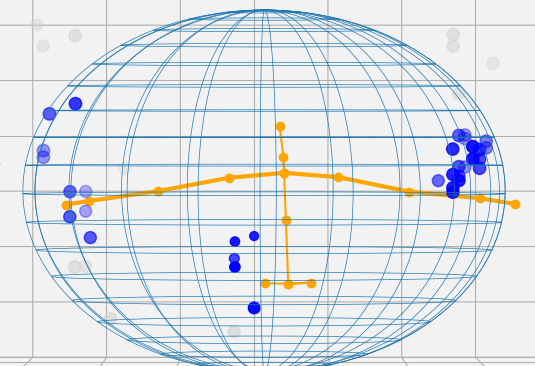
\includegraphics[width=0.9\linewidth]{figures/internal data/IAmMuse internal view.png}
        \caption{Internal data view}
        \label{figure: internal data view, a}
    \end{subfigure}
    \begin{subfigure}{0.5\textwidth}
        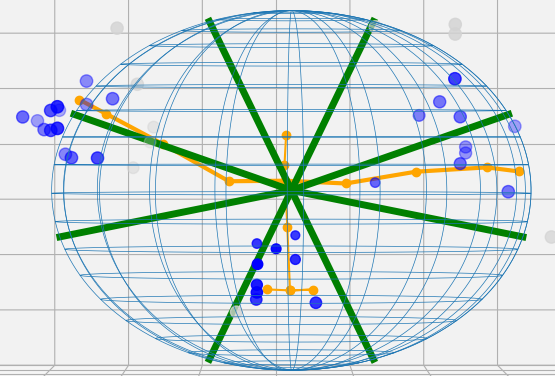
\includegraphics[width=0.9\linewidth]{figures/internal data/IAmMuse internal view with zones.png}
        \caption{Internal data view with zones}
        \label{figure: internal data view, b}
    \end{subfigure}
    
    \caption{Internal data view}
    \label{figure: internal data view}
\end{figure}
% \textbf{¡¡¡¡ The explanation is quite difficult to follow currently, think up specific terms and meanings, in order to make the explanation more clear!!!}\\
% Things to get a specific term for
% \begin{itemize}
    % \item MEB center
    % \item MEB radius
    % \item MEB circle (for reasoning)
    % \item specific arm zones, e.g. left low; left mid; left high; right low...
    % \item angle ranges
% \end{itemize}

The method used for data interpretation is tightly linked to the method used for data enhancement, since the data enhancement method adds a specific type of information to our input data.
In the case of IAmMuse, we have the ball, which encompasses the user, as well as the extra dimension of weight, added to the point cloud.
The data interpretation method of IAmMuse will thus be built around this new information.
A visualization of this internal state, with the ground truth in orange, is shown in \cref{figure: internal data view}.


\subsection{Conceptually}
\label{sub-section: tracking method - data interpretation - conceptually}

% What do we want to predict
As was mentioned at the start of \cref{chapter: tracking method}, the goal of IAmMuse is to predict what \textit{zone} a specific hand is in.
These zones are defined as being a \textit{range of angles}, and can be either "low", "middle", or "high". 
Respectively representing situations where the user points at the floor, outwards, or at the sky.
% 2D simplification.
When reasoning about this system, a useful simplification is to think about the system in two dimensions.
This would change our enclosing ball into a circle, enclosing the movement space of the user's arm, where the center of the circle is still at the user's sternum, and the edge still traces the potential positions of the user's hands. 
Each 3D point would then be transformed into its 2D projection, where we remove the direction outwards from the mmWave camera.
The reasoning performed on this simplified model still holds in the actual model, why this is the case will be specified throughout \cref{sub-section: tracking method - data interpretation - practically}.


% pointcloud -> angleset
Since each point can be interpreted as a prediction/reading of the position of the arm, it's also possible to determine a prediction/reading of the angle of the arm, as predicted by that singular point.
This \textit{point angle} can be defined as the angle of the line which goes from the user's sternum (center of the enclosing circle) to that specific point.
This allows us to transform our weighted pointcloud into a set of predicted angles, with a weight equal to the original point weight, which represents the "value" of that particular prediction.
With this list of weighted angles, it's now easy to make some likelihood predictions for specific arm zones by simply looking at the zone in which each angle falls and the weight of that angle.


\subsection{Practically}
\label{sub-section: tracking method - data interpretation - practically}

% Pointcloud -> angleset
The first step that needs to be performed is to transform the weighted point cloud into a set of weighted angles, corresponding to the angle which the arm would have if it went through the specific point.
To calculate this angle, the vector between the center of the enclosing ball and the specific point considered is taken.
Then the arc-tangent of this vector's distance in the X-axis (side to side) and the Z-axis (up-down) is considered to be the angle of the point.
Since the user is expected to hold their arms out mostly straight, the user can be correctly assumed to be roughly two-dimensional.
From this, we can see that the encompassing ball can be viewed as an encompassing circle, since the center of the circle is said to be at the location of the user's sternum, and is thus at the same distance from the mmWave camera as the user.
% \textbf{INCLUDE THIS?}
A better method would have been to consider the angle between the aforementioned vector and the down vector, making a distinction between "left" and "right" based on the sign of the X component of the vector.
This would allow the user to hold their arms somewhat more forward without affecting the accuracy of the system.
In this case, the simplified two-dimensional reasoning still applies, as you can take an X-value in the 2D space as being $\sqrt{x^2 + y^2} \times \text{sign}(x)$.
% \textbf{END OF INCLUDE THIS?}
Doing this for all points in the weighted point cloud yields us a list of angles with an associated weight.

% angleset -> prediction
Each arm zone is internally defined as a range of angles, where a zone should thus be selected if the specific arm is within that specified angle zone.
The way IAmMuse differentiates between the left hand and the right hand is simply by the angle.
These angles exist on a range between $0\degree$ and $360\degree$, where $0\degree$ is down, $90\degree$ is left, $180\degree$ is up, and $270\degree$ is right. 
In this way, systems can be generalized over both arms.
Each arm zone then gets a weight equal to the cumulative weight of all the angles that fall within its angle range, only considering angles from one frame.
The right and left zones with the highest weight are then predicted to be the zone where the user's hands are currently.
Making sure only to select \textit{one} left zone and \textit{one} right zone.

% Why we need stabilization
% This system has a few issues, though. 
% For one, very sparse frames currently have the same effect as very dense frames, while the information present in a sparse frame is, by definition, lower.
% Since the mmWave radar has frames where it simply produces less, and less useful data, it often happens that a small bit of noise will produce an almost random prediction on these frames.
% Even on denser frames, it's possible for large noise spikes to poison a specific prediction.
% Lastly, there is the issue where an arm located at the edge of two zones will be predicted to be one or the other almost at random for any particular frame, due to the inherently random point distribution point samples generated by the mmWave radar.
% While this is not a big deal when it comes to a single frame, during system usage, this means that the system might rapidly change its prediction back and forth, resulting in a non-stable output on a stable input (user arm position), which is a bad thing.
% For these reasons, it's important to consider methods for data stabilization.

\subsection{Data Stabilization}
\label{sub-section: tracking method - data interpretation - data stabilization}

% stabilization intro & minimal points
There are a few issues with the current system, though, all to do with the stability of the resulting prediction, and extra systems have been put in place to mitigate these issues
Firstly, one issue occurred when the mmWave radar produced very sparse frames. 
Sparse frames contain disproportionately few points, and thus also contain disproportionately few signal points. 
This means that the predictions of IAmMuse are more susceptible to the random variations in the point distributions, as well as being more susceptible to noise, since the prediction system simply looks at which zone has the highest weight.
The way in which IAmMuse mitigates this issue is by setting a \textit{minimal weight} which a zone must have to be considered as a "valid prediction", if no valid prediction was made for a side, the previous prediction is kept.
This mitigation strategy does have the side effect of ignoring some frames if they are too sparse, but this isn't a huge problem, as the amount of information present in that frame was already very low, by way of how sparse it was.
A solution that adds the data from these "missed frames" to the following frames could be made.
This would increase the amount of information the system uses, but could also induce a lower responsiveness by taking into account stale information.
For these reasons, such a system was not put in place in IAmMuse.


% Multiple predictions needed
Another similar issue occurs when a large spike of noise is perceived for a single frame, this influx of faulty data can make the system select an incorrect zone.
These large noise spikes do not happen regularly, but they happen often enough that a mitigation system was useful.
In these cases, most frames in a sequence will give a similar result, but one frame will give a "faulty prediction".
Since we know that, in a correct set of frames, the same zone would likely be predicted multiple times in a row, as the user's arm stays in that zone, we can filter out the faulty case by only choosing a new zone if that zone has been predicted twice in a row.
In this system, it's important not to count "missing predictions" (as specified in the previous paragraph) as a part of these consecutive predictions.
This system does add some delay to the selection of a new zone, specifically 100ms if you receive correct predictions every frame. 
For the IAmMuse system, this delay is a worthwhile tradeoff for the added stability against both noise and random fluctuations in the mmWave radars' output, but this may not be the case for every system.

% Zone expansion
Lastly, IAmMuse had to solve an issue in the scenario where a user is holding their arm near the border of two zones.
In this case, IAmMuse may predict either zone at random, purely due to the random nature in which the points in a mmWave frame are distributed.
While a singular frame prediction would not be incorrect per se, the fact that the system produces an unstable output while the user provides a stable input (a stationary arm) is incorrect.
The way that IAmMuse solves this issue is by expanding the region assigned to the currently selected zone.
This eliminates the issue, as the randomly distributed points that are on the edge of the two zones will be predominantly in the active zone if the zone's angle range is increased.
In IAmMuse, the active zone's angle range is increased by $10\degree$, or $5\degree$ on each side, and neighboring zones are shrunk in accordance.
This increase should be as small as possible while still providing the stability-increasing effect.
During system design, an increase of $10\degree$ seemed to be the smallest amount that fulfilled this wish.





% The data interpretation method is often tightly linked to the data enhancement method used, as we will use the extra context provided by the data enhancement in the interpretation.
% In the case of IAmMuse's final system, the extra context we've been given is the MEB, providing us with a rough center point of the user, as well as an estimation of the outer reach of their arms.
% % simplify to 2d explained
% During the design and explanation of the interpretation algorithm, we will often simplify the user's points to be on a plane, rather than in 3d space. 
% The MEB would then likewise be considered to be a circle, with the center still at the user's sternum, and the edge tracing the path the user's hands can trace (assuming outstretched arms).
% This estimation makes the reasoning a lot more intuitive. At the end of the section, we will also briefly touch on why this reasoning also extends to our actual system, which does operate in 3d space, rather than 2d space.
% % continue
% The main idea which is used in the interpretation of the data is that the angle of the arm is very closely modeled by looking at the angle between the sternum and a user's hand.
% The sternum position is already known to be roughly at the center of the MEB, and the user's hands are known to be roughly at the edge of the MEB circle.
% This transforms our problem of "find the angle of the arms" to "find the position of the hands on our circle", which turns out to be a lot simpler.
% 
% To find the angle of the arms, a few things need to be done: points that belong to the hand should be specified, these points should be placed on the MEB circle, the angles between these points and the MEB center should be calculated, and this set of angles should be transformed into a hand/arm angle prediction.
% The first step is done in a somewhat different way. 
% We know that the points at the circle edge tell us a lot of things about the position of the hands, and the further away a point is from that circle edge, the less we trust the information. 
% Since your arm position tells you something of where the hand is, but your torso won't tell you anything.
% For this reason, each point is given a \textit{weight}, dependent on its distance to the circle edge.
% In practice, this is achieved by taking the distance between a point and the MEB center, and applying the Gaussian function to this distance, where $\mu$ is the radius of the MEB, $\sigma^2$ is taken to be $0.25$, and x is the previously mentioned distance.
% The output of this function is used as a weight of the point, which is representative of "how hand-like" the point is.
% Calculating the angle for each point is a trivial trigonometric function, and will leave us with a set of angles with weights.
% 
% The last part of the interpretation is turning this list of angels and weights into two final arm positions, one for the right arm and one for the left arm.
% In this thesis, we do not care about the exact arm position, rather, we care about the "region" where the arm currently is.
% This region is specified as being "low", "middle", or "high", which are simply ranges of angles in which the arm can be.
% The fact that the system is expected to generate an output region can be used in the interpretation.
% To find out the likelihood of an arm being present in a specific region, you can look at the "weight" of said region, where a region's weight is the sum of the weights of all points (angles) that exist in that region.
% In this manner, a frame-specific prediction for the arm location can be generated by selecting the zone with the highest weight on each side (left, right).
% One problem with this approach is that the output is very unstable.
% 
% A few methods are used to stabilize the output of the arm location predictions.\\
% Firstly, the arm position (low, mid, high) that is currently selected will increase the angle range that it considers "its region" by $5\degree$ on each side. 
% e.g. the middle zone usually considers points "in its zone" when their angle is between $65\degree$ and $105\degree$, but if the middle zone is already selected, it will now consider angles between $60\degree$ and $110\degree$, this region increase will shrink the other regions.
% This system avoids the situations where a user's arm is "on the edge" of two zones and rapidly changes which zone is predicted while the user keeps their arm still.\\
% Secondly, there is a certain threshold weight that a zone needs to achieve to be considered as a "valid zone contender", this makes sure that very sparse frames can not trigger a faulty zone change based on only a few points.\\
% Lastly, a specific zone is only selected as the actual zone if it was predicted to be the correct zone twice in a row.
% Note that some frames may not have any predictions at all if none of the zones crossed the weight threshold, in this case, no prediction was made, thus it does not impede a zone from being chosen twice.
% e.g. \textit{frame n}, zone left low is selected. \textit{frame n+1} no zone is selected. \textit{frame n + 2} zone left low is selected.
% In this situation, \textit{left low} has been selected twice in a row, thus, the zone gets set to left low.
% 
% Earlier in the section, it was stated that we could reason about the minimal enclosing ball as if it were a circle, the reasons for this assumption will be given here.
% First off, during the usage of the system, the user is expected to stand facing the FMCW, with their arms out to the side, lifting or lowering them.
% In this situation, the point cloud produced by the user falls roughly in a plane where we simply ignore the y direction, thus, for the points belonging to the user, the simplification to a circle is valid.
% Furthermore, the number of noise points that still exist in this part of the pipeline is small, and given the spatial distribution observed from these points, the likelihood of one of these points being present near the edge of the ball but in front of or behind the user is very slim.
% Therefore, only outlier points will ever appear near the edge of the ball while not being well modeled by the circle.
% Points that are at a large distance from the edge of the ball will be disregarded automatically by being assigned a low weight, as the distance between the centroid and the specific point can be (and is) calculated in 3d.
% Due to the above given reasons, there is no feasible situation in which the assumption (for reasoning purposes) of a circle does not apply accurately to our actual ball.
% Lastly, it's important to mention how we get the "angle" between two points now, given that we are not actually using 2d coordinates in the system.
% The angle of the arm is considered to be the angle between the down vector and the vector that goes from the MEB circle to the point in question.
% This has the added benefit that users are allowed to hold their arms at a somewhat forward angle if this is more comfortable for them, and the calculation still holds true in the same manner.



% % This section describes HOW we do the data interpretation, given the different systems described above, specifically the minimal enclosing ball.
% % This includes the general high-level overview of the system, including zones on the MEB, filtering, and processing.
% % It will also discuss different smaller systems, such as the active zone size increasing code, the stabilization code, which requires a zone to be selected more often, and will discuss the concept of "weight" in the various system contexts.
% % 
% % \textbf{We use a ball, not a circle, explain}

% Create a chapter describing test setup, baseline and the datasets
\chapter{Setup, Baseline and Dataset}
\label{chapter: setup baseline dataset}


% Create an evaluation
\chapter{Evaluation}
\label{chapter: evaluation}

\section{Baseline Analysis}
\label{section: evaluation - baseline analysis}

Show the results of mars trained on the calib data of ONLY that specific recording

\section{Larger Models}
\label{section: evaluation - larger models}

Describe the new MARS trained models we'll be evaluating, (\texttt{mars\_paper} and mars trained on \textbf{all} calib data)

Show their results, and explain why they perform badly (overfitting, non-representative data).


\section{IAmMuse vs Best MARS}
\label{section: evaluation - iammuse vs best mars}

Describe how we'll train the best MARS model we could make.

Show the acuracy results, discuss how it is better then the previous mars' but still worse then IAmMuse

Show the time-prediction diagram (showcasing the "stuttering" of mars)

Show that the lowpass MARS results still underperform.

Mention that, even when given all the tools we could, mars could not perform better then IAmMuse

% Create conclusions
\chapter{Conclusion}
\label{chapter:conclusion}

% \input{mainmatter/5. conclusion/5.1. findings}

% \input{mainmatter/5. conclusion/5.2. limitations}
% \section{Findings}
% \label{section: conclusion - findings}
% Quickly summarize the main findings which were discussed in \cref{section: discussion - implications}.

To summarize … Add a summary of the findings 


\section{Recommendations/Future work}
\label{section: conclusion - future work}
Depending on the results, I either want to encourage more research into stochastic MMWave interpretation, both in breath and scope. aka, people should try and make stochastic systems for more complex problems/different problems. And people should look further at optimizations in the current system, in firmware used, system tuning, and potential broadening.
An interesting problem would be to see if you can increase the amount of zones, and reduce them in size, in such a way that you have ~20 zones per side, and to then try and modify the system to still predict zones correctly.
This could be achieved with a kind of "decaying charge" (each step the zone loses a percentage of its value) and a kernel/distance based "charge addition" (each point gives value to multiple zones, depending on how "near to it" they are).


\subsection{Dynamic Initialization Recalculation}
The initialization step is currently fully static, this could be adapted to become a more dynamic system.

\subsection{More Continuous Result Angles}
One shortcoming of the current system is that it only considers some broad angle-zones.
This isn't a weakness in and of itself, but it limits the usefulness of the system.
One way to potentially mitigate this issue is to change the data interpretation method described in \cref{section: tracking method - data interpretation} to allow for a broader range of output values.
One manner in which that could be done is to consider 360 "zones" of $1\degree$ each. 
Due to the relatively low point density, this system would need to solve the issue that it's very unlikely for multiple points to end up in the same zone (which would make the system prone to random data distribution artifacts), and the fact that the current stabilization methods would not work anymore.
One way to solve the first issue would to to have each point add its "weight" to many zones "near" it, for example, by using a Gaussian kernel to distribute its weight across nearby zones.
This would produce a likelihood-density distribution along the angle axis.
The peaks would be representative of where the arms might be, some clever new stabilization methods would be needed for this system, to ensure that "one sided frames" (frames whose data is predominantly on one side) don't mess things up, as well as to stabilize the output in general.

One potential idea is to add the new weights to a running sum (for each zone) and normalize the output on a specific "Total weight", e.g., at the end of the normalization the sum total of all zone weights should always be 30.

However, the further design and testing of these systems will be left to any future researchers.



% Create future work
% \chapter{Future Work}
\label{chp:futurework}

Future work.

% Create bibliography
% Natbib has been configured to be visually the same as `plain`, when using `plainnat`.
\bibliographystyle{plainnat} % use plainnat, with visuals exactly the same as plain
% \bibliographystyle{plain} % Please do not change the style of bibliography (yes, it should be `plain`)
\bibliography{bib/MyMScTUDESThesisBibFile} % remove "../" before "bib" if you compile directly in Overleaf or in your favourite local LaTeX distribution

% Create appendix
\appendix
% \crefname{chapter}{appendix}{appendices}
% \Crefname{chapter}{Appendix}{Appendices}

\chapter{Standardized Movement Set}
\label{appendix: standardized movement set}

In order to get similar data across users, and to make sure that all movements where performed, a standardized movement set was divised.

Each position was held for 2-3 seconds. 
Each row in the table shows a \textit{left hand position} and a \textit{right hand position}, which can both be either "L" for low, "M" for middle, or "H" for high.


\begin{table}[h]
    \centering
    \begin{subtable}%[t]%{0.2\textwidth}
    \centering
    \begin{tabular}[t]{||c|c|c||}
    \hline
    Step & Left & Right\\
    \hline \hline
      1 & L  & L\\
      \hline
      2 & M  &M\\
      \hline
      3 & H & H\\ 
      \hline
      4 & M & M\\ 
      \hline
      5 & L & L\\ 
      \hline
      6 & L & M\\ 
      \hline
      7 & L & H\\ 
      \hline
      8 & L & M\\ 
      \hline
      9 & L & L\\ 
      \hline
      10 & M & L\\
      \hline
      11 & H & L \\
      \hline
      12 & M & L \\
      \hline
      13 & L & L \\
      \hline
      14 & M & M \\
      \hline
      15 & M & H \\
      \hline
      16 & M & M \\
      \hline
    \end{tabular}
    \end{subtable}
    \begin{subtable}%[t]%{0.2\textwidth}
    \centering
    \begin{tabular}[t]{||c|c|c||}
    \hline
    Step & Left & Right\\
    \hline \hline
      17 & M & L \\
      \hline
      18 & M & M \\
      \hline
      19 & H & M \\
      \hline
      20 & M & M \\
      \hline
      21 & L & M \\
      \hline
      22 & M & M \\
      \hline
      23 & H & H \\
      \hline
      24 & H & M \\
      \hline
      25 & H & L \\
      \hline
      26 & H & M \\
      \hline
      27 & H & H \\
      \hline
      28 & M & H \\
      \hline
      29 & L & H \\
      \hline
      30 & M & H \\
      \hline
      31 & H & H \\
      \hline
    \end{tabular}
    \end{subtable}
    \caption{Standardized movement set}
    \label{fig: standardized movement set}
\end{table}

\chapter{User Explanation}
\label{appendix: user explanation}

The users were given a small \textit{explanation pamphlet} before using the system.
This and the next page show that pamphlet. 

% Double separation line and spacing
\vspace{2em}
\hrule
\vspace{0.2em}
\hrule


\includegraphics[page=1, trim = 25mm 140mm 7mm 20mm, clip, width=1\textwidth]{figures/experimental setup/mmwave experiment explanation.pdf}

\includegraphics[page=2, trim = 25mm 30mm 7mm 20mm, clip, width=1\textwidth]{figures/experimental setup/mmwave experiment explanation.pdf}
\chapter{Experiment Notes}
\label{appendix: experiment notes}

During the experiment, I took some notes on how different people performed good or poorly (in my subjective view).

% Double separation line and spacing
\vspace{2em}
\hrule
\vspace{0.2em}
\hrule

General
Its interesting to look at how experience effects the accuracy of my system AND of Mars DL system, and to see if one might be better with more experienced users.

IDEA: more lenient noise filtering might bring better results with general users, as their arm pointcloud might not be present in as many frames as with more experienced users. 
e.g. Considering 5 frames as opposed to 3 frames in the temporal filtering may increase performance on general users.

The chip seemed to be mounted not perfectly level, with the left part (from the users viewpoint) being ever so slightly too high

User 61
The fact that user 61 had never used the system was quite visible. 
The system has a decent bit of nuance which should be known for effective use, and was not known by the user.
We did 3 standard runs, during the first they barely wove their hands, after that I reminded them that the system works best when you wave your hands, then they moved them up and down quickly (5-10 Hz) or to and from the camera, but with large movements (1-3 Hz).
The third standard run I specified that small movements back and forth towards the camera are best, which resulted in jazz hands.

In the free play sections they experimented with still arms and arms moving to and from. However it seemed like the configuration has their body put a bit too high, as they had difficulty hitting the high notes.

User 94
User 94 had a decent understanding of the system from the get go, but between standard run 1, 2, 3 I still gave them some small tips on how to better use the system.

In standard 2 they moved the wrong arm on a few occasions.


They where also enthusiastic to try the free play section of the experiment.
User 41
In the first standard run they didn’t move their arms a lot, between run 1 and 2 I informed them of the effective methods of moving your arms (for higher data collection), they tried following it, but did not do so consistently.
Between set 2 and 3 I informed them how to have their arms “good”in the zones (as “low”is less low then most think).


User 7
Had some difficulty with the movements.


User 51
They often held their low positions very low, and their high positions very high, which caused some accidental incorrect triggers.

I gave the the advice of moving their hands more (jazz hands) after the first trial, and told them that low wasn’t quite as low as they put it (though they didn’t improve significantly).

In general they had fun and where enthusiastic, but didn’t move their hands a lot, or if they moved they moved their whole arm, and they held high “very high”and low “very low“

User 52
after the first trial I told them about the zone locations and waving, I once again reminded them about that after the second trial, they did try to wave their hands well.
One thing was that it felt like they might’ve been a bit too tall for how I had the system setup, as the center of the MEB seemed to be nearer their chin then their sternum.

\chapter{Recording Frame Distribution}
\label{appendix: recording frame distribution}

The different recordings have a different number of frames in total, and will also use a different number of frames for the \textit{pre-configuration} step. 
The following table shows the exact number of frames used for \textit{pre-configuration} as well as the number of frames used for \textit{evaluation} (evaluation frames = total frames - preconfig frames).

The table will use a shorthand notation to refer to recordings.
Standard movement set recordings will be specified with 'std' while free play recordings will be specified with 'free'.
The user of which the recording is will be specified by 'usr\_xx'.
The specific recording will be specified with 'rec\_a/b'.
Examples:
\begin{itemize}
\item "\textbf{standard movement set} recording from \textbf{user 07} number \textbf{2 out of 3}" becomes "std usr\_07 rec\_2/3"
\item "\textbf{free play} recording from \textbf{user 52} number \textbf{1 out of 1}" becomes "free usr\_52 rec\_1/1"
\end{itemize}


\begin{tabular}{|c|c|c|}
    \hline
    \textbf{Recording} & \textbf{\# Pre-configuration frames} & \textbf{\# Evaluation frames} \\
    \hline
    \textit{total} & 7229 & 40272 \\
    \hline
    free usr\_07 rec\_1/2 & 168 & 853 \\
    \hline
    free usr\_07 rec\_2/2 & 171 & 1014 \\
    \hline
    free usr\_0 rec\_1/1 & 179 & 331 \\
    \hline
    free usr\_41 rec\_1/1 & 235 & 1423 \\
    \hline
    free usr\_51 rec\_1/4 & 187 & 1322 \\
    \hline
    free usr\_51 rec\_2/4 & 206 & 1478 \\
    \hline
    free usr\_51 rec\_3/4 & 208 & 1461 \\
    \hline
    free usr\_51 rec\_4/4 & 179 & 1431 \\
    \hline
    free usr\_52 rec\_1/2 & 223 & 668 \\
    \hline
    free usr\_52 rec\_2/2 & 183 & 863 \\
    \hline
    free usr\_61 rec\_1/2 & 194 & 1247 \\
    \hline
    free usr\_61 rec\_2/2 & 180 & 769 \\
    \hline
    free usr\_94 rec\_1/2 & 190 & 861 \\
    \hline
    free usr\_94 rec\_2/2 & 230 & 1412 \\
    \hline
    std experienced\_user rec\_1/3 & 171 & 1003 \\
    \hline
    std experienced\_user rec\_2/3 & 210 & 1043 \\
    \hline
    std experienced\_user rec\_3/3 & 162 & 917 \\
    \hline
    std usr\_07 rec\_1/3 & 232 & 905 \\
    \hline
    std usr\_07 rec\_2/3 & 246 & 1132 \\
    \hline
    std usr\_07 rec\_3/3 & 211 & 1203 \\
    \hline
    % std usr\_0 rec\_1/2 & 152 & 1074 \\
    % \hline
    % std usr\_0 rec\_2/2 & 108 & 1021 \\
    % \hline
    std usr\_41 rec\_1/3 & 182 & 1134 \\
    \hline
    std usr\_41 rec\_2/3 & 206 & 1150 \\
    \hline
    std usr\_41 rec\_3/3 & 223 & 1204 \\
    \hline
    std usr\_51 rec\_1/3 & 191 & 1117 \\
    \hline
    std usr\_51 rec\_2/3 & 212 & 1181 \\
    \hline
    std usr\_51 rec\_3/3 & 182 & 1212 \\
    \hline
    std usr\_52 rec\_1/3 & 204 & 989 \\
    \hline
    std usr\_52 rec\_2/3 & 189 & 1147 \\
    \hline
    std usr\_52 rec\_3/3 & 198 & 1028 \\
    \hline
    std usr\_61 rec\_1/3 & 183 & 1118 \\
    \hline
    std usr\_61 rec\_2/3 & 151 & 1291 \\
    \hline
    std usr\_61 rec\_3/3 & 167 & 1017 \\
    \hline
    std usr\_94 rec\_1/3 & 275 & 1067 \\
    \hline
    std usr\_94 rec\_2/3 & 223 & 1142 \\
    \hline
    std usr\_94 rec\_3/3 & 218 & 1044 \\
    \hline
\end{tabular}

\chapter{Failed Methods}
\label{app: failed methods}


This appendix describes the methods for algorithmic HPE which have been attempted, but did not succeed in producing good enough results.


\end{document}


% [[ TODO ]]
% List of things still needing figuring out.
%
% - Appendix references: currently `cref` references appendixes as 'chapters', which is an issue.